The Earth stands at a critical juncture in its history, where the consequences of human activity on the environment have reached a crossroads of global significance. Climate change, driven primarily by the relentless emission of greenhouse gases, has manifested itself in increasingly severe weather patterns, rising sea levels, and ecological disruptions. The urgency of the situation cannot be overstated, as nations grapple with the complex challenge of reducing carbon dioxide (CO$_2$) emissions to mitigate the impending climate crisis \cite{solomon2009irreversible,noaa-co2,world2016ambient}. 

The dire need for sustainable energy solutions has never been more evident. Various sectors of the economy are challenged to reduce their carbon footprint in order to restrict their impact on climate change. The transport sector was responsible for 23\% of global emissions from fuel combustion in 2021 \cite{iea-transport} and emerges as a critical contributor to the climate change predicament. 

\begin{figure}[h]
    \centering
    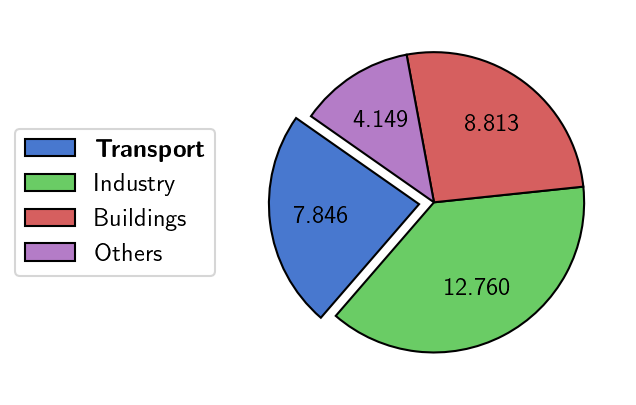
\includegraphics[width=0.75\textwidth]{Images/Chapter1/iea-transport.png}
    \caption{2021 Global CO$_2$ emissions from fuel combustion by sector [$\text{GtCO}_2$]. Source: IEA (2023) \cite{iea-transport}.}
    \label{fig:iea-transport}
\end{figure}

As societies evolve and the global population continues to grow, the demand for transportation, particularly in the form of automobiles and other fossil-fuel-reliant means, has risen dramatically. Innovative solutions are crucial to decouple the connection between personal mobility and CO$_2$ emissions. Electric vehicles (EVs) have emerged as a promising alternative to traditional internal combustion engine vehicles. They offer the potential to revolutionize the way we commute, significantly diminishing the transportation sector's contribution to carbon emissions. 

% \begin{figure}
%     \centering
%     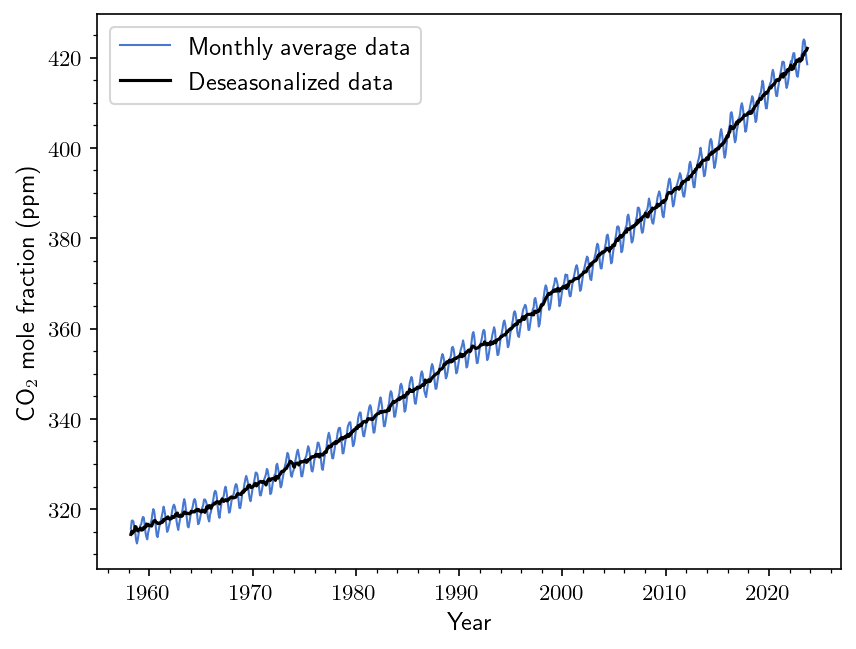
\includegraphics[width=0.7\textwidth]{Images/Chapter1/noaa-co2.png}
%     \caption{Trends in Atmospheric Carbon Dioxide. Source: NOAA (2023) \cite{noaa-co2}.}
%     \label{fig:noaa-co2}
% \end{figure}

At the heart of the electric vehicle industry's transformation lie lithium-ion batteries (LIBs). These energy storage devices have rapidly gained prominence as the primary means of powering EVs \cite{zubi2018lithium,stampatori2020li}. The suitability of LIBs for this role is driven by their impressive energy density, rechargeability, and relatively low environmental impact compared to conventional fossil fuels \cite{korthauer2018lithium}. As we explore the potential of lithium-ion batteries, it becomes evident that their development and adoption may hold the key to mitigating the environmental impact of the transportation sector. 

% This part has to be changed since it is copied from (Failure description: 890)
The shortcomings of LIBs are their narrow operational temperature range and charge-discharge rates. The capacity of the battery degrades faster if working at a high temperature, and the lifetime is shortened, too \cite{ma2018temperature,ning2003capacity}. When LIBs adre subjected to conditions outside of their design window, they may fail through a rapid self-heating or thermal runaway, which may ignite the sorrounding materials \cite{palacin2016batteries}. 
% This part has to be changed since it is copied from (Matilda Thesis)
Hence, LIBs require meticolous safety testing in order to guarantee safe use in all usage frameworks. Safety tests must produce reliable parameters to enable satisfactory evaluation and classification of safe battery specifications. The consumer and industrial market demands safe, low-cost, high-power batteries produced with low environmental impact, using sustainable components that enable easy recycling \cite{doughty2012general}.

In the following section the functioning of Lithium-ion batteries is described, followed by a discussion of the safety and degradation issues that arise in LIBs.

\section{Overview}
\label{sec:overview}
\cite{korthauer2018lithium,goodenough2013li}
\subsection{Anode}
\label{sec:anode}

\subsection{Cathode}
\label{sec:cathode}

\subsection{Electrolyte}
\label{sec:electrolyte}

\subsection{Separator}
\label{sec:separator}

\subsection{Current Collectors}
\label{sec:current-collectors}

\subsection{Cell Geometries and Designs}
\label{sec:cell-geometries-designs}

\section{Safety and Degradation}
\label{sec:safety-degradation}
